\chapter{Survey one results and analysis}
\label{chap:Survey one results and analysis}
\lhead{\emph{Survey one results and analysis}}
This chapter will show the visuals of the results from both surveys conducted, the first section will be the professional educator survey results and the second survey will be the Autism and Assistive Technology Survey. Each survey will be followed by a table to give overall and interesting feedback from the respective survey conducted.

\section{Survey one results}

Survey one  is the professional educator Survey, this survey involved 24 participants who all had experience educating individuals with Autism. The participants occupations included home educator, special needs teacher, speech and language therapist, additional needs educator and various other professional educator roles.

\begin{figure}[ht]
\centering
\includegraphics[width=1.0\textwidth]{IDD_LauraMartin_R00124705/Figures/1.png}
\caption{Occupation answer box }
{For question one, 24 participants best described their occupation in the field of professional education.}
\end{figure}

\begin{figure}[ht]
\centering
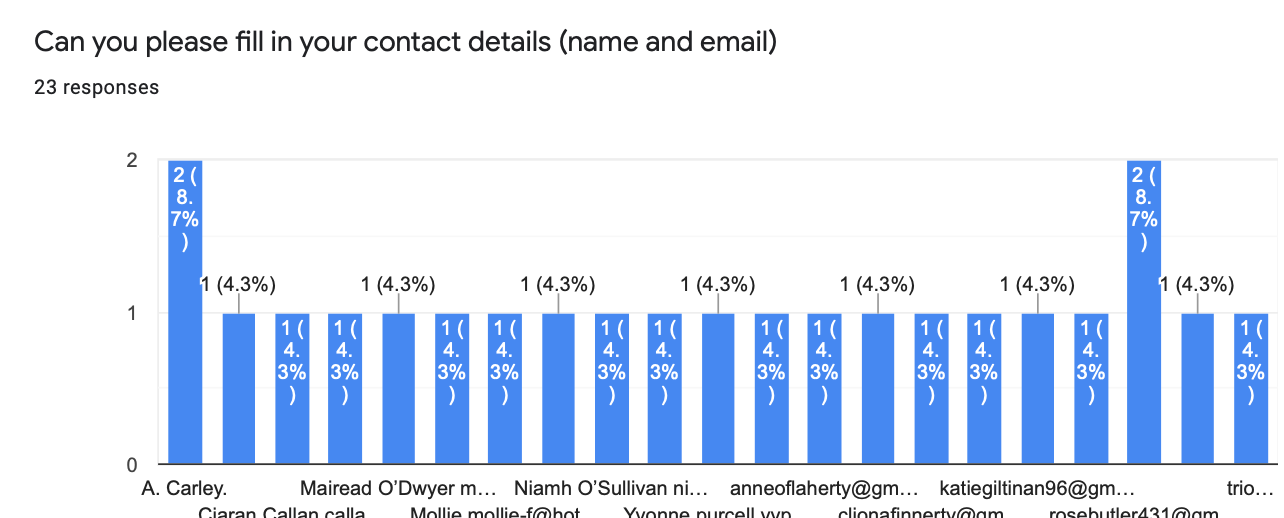
\includegraphics[width=1.0\textwidth]{IDD_LauraMartin_R00124705/Figures/2.png}
\caption{Details of participants}
{For question two, 23 respondents gave their name and email addresses.}
\end{figure}

\begin{figure}[ht]
\centering
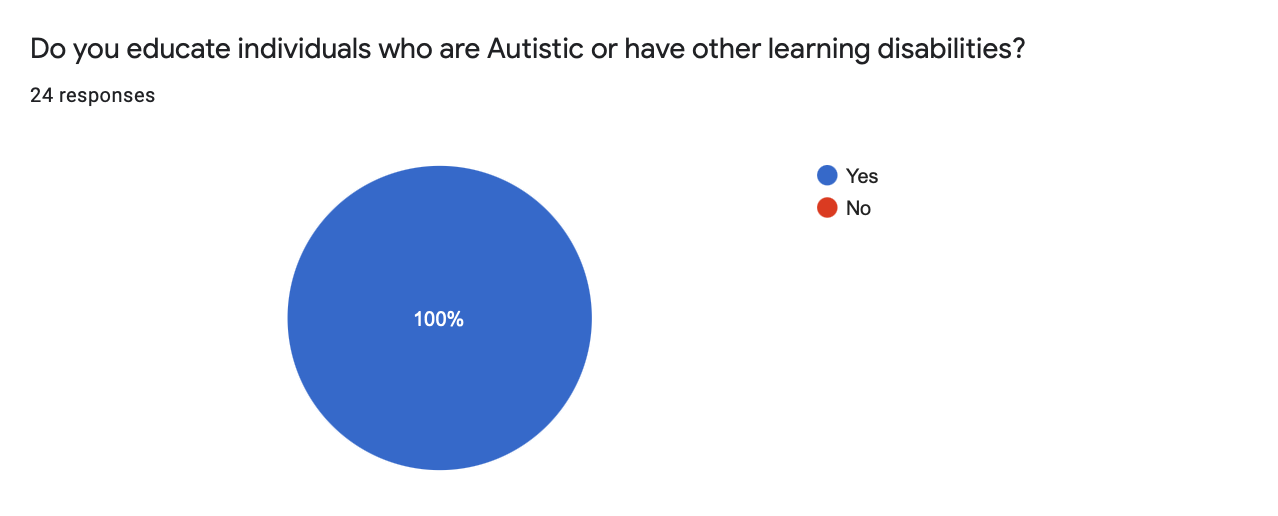
\includegraphics[width=1.0\textwidth]{IDD_LauraMartin_R00124705/Figures/4.png}
\caption{Pie chart representing the participants involvement of educating individuals with Autism}
{For question three, 24 respondents gave their experience educating individuals with Autism.}
\end{figure}

\begin{figure}[ht]
\centering
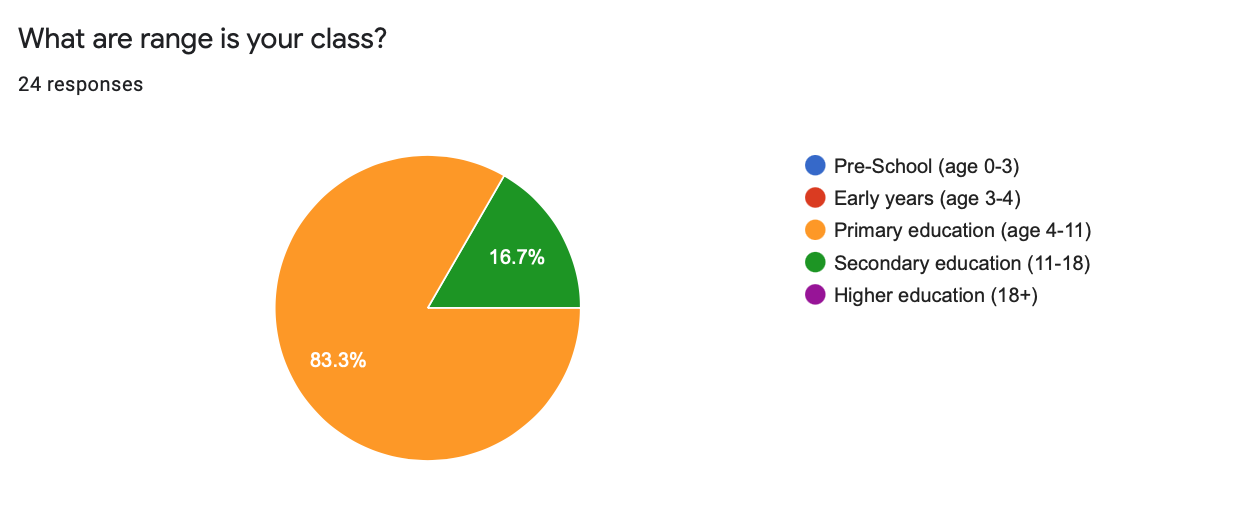
\includegraphics[width=1.0\textwidth]{IDD_LauraMartin_R00124705/Figures/5.png}
\caption{Pie chart representing the participants class age range}
{For question four, 24 respondents gave the age range of their class, age 4-11 being the most popular age range and followed by 11-18 years old.}
\end{figure}

\begin{figure}[ht]
\centering
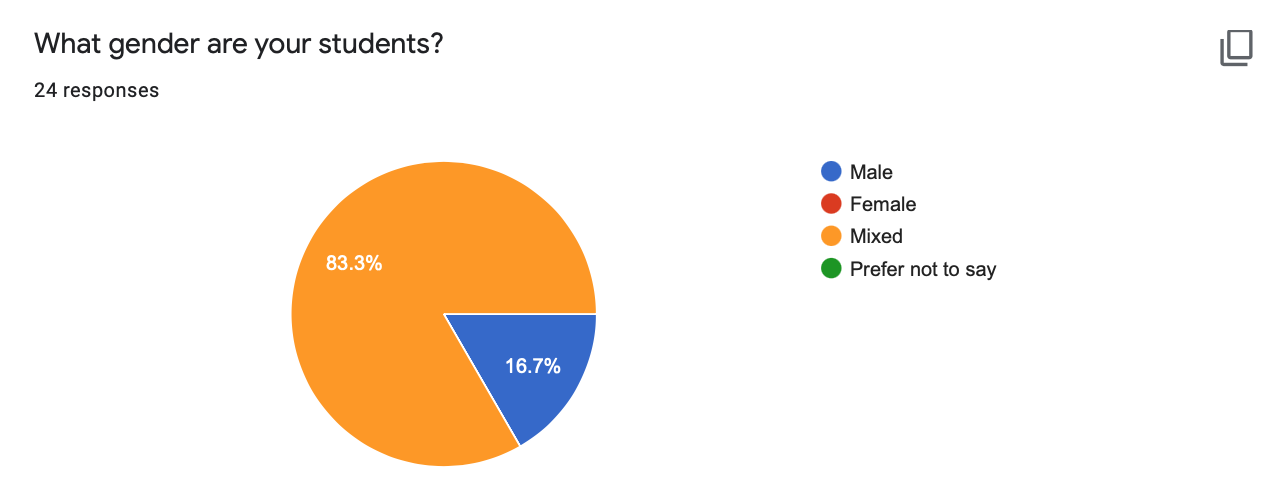
\includegraphics[width=1.0\textwidth]{IDD_LauraMartin_R00124705/Figures/6.png}
\caption{Pie chart representing the participants genders in their classroom}
{For question five, 24 respondents gave the gender of the students they had in the classroom, mixed being the most popular answer, followed by a full male classroom.}
\end{figure}

\begin{figure}[ht]
\centering
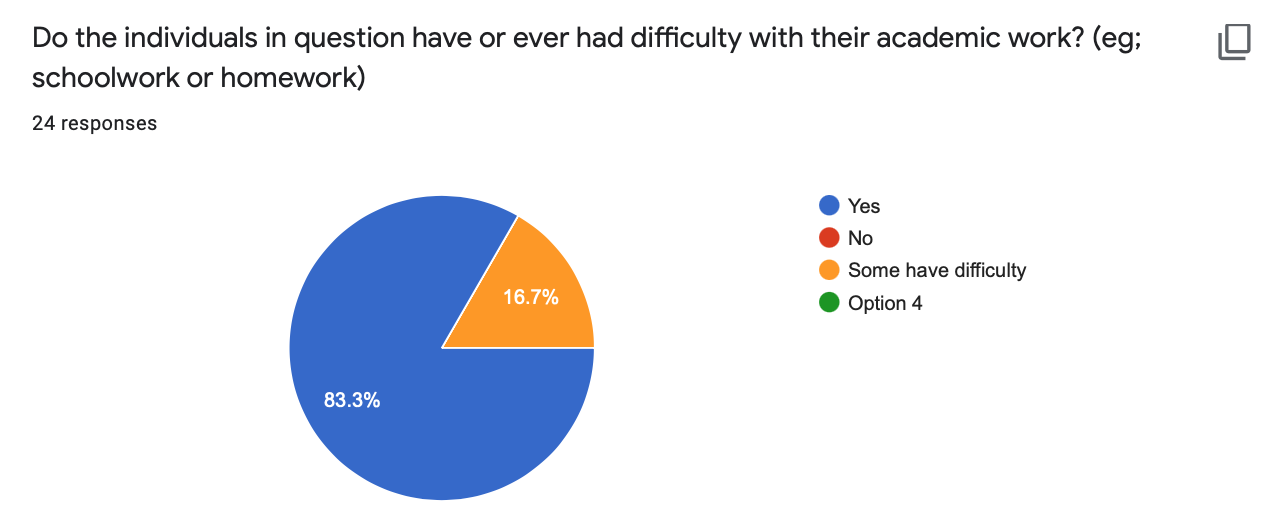
\includegraphics[width=1.0\textwidth]{IDD_LauraMartin_R00124705/Figures/7.png}
\caption{Difficulty with academic studies pie chart}
{for question six, 24 respondents were given a multiple choice question about their students having difficulty with academic studies.}
\end{figure}

\begin{figure}[ht]
\centering
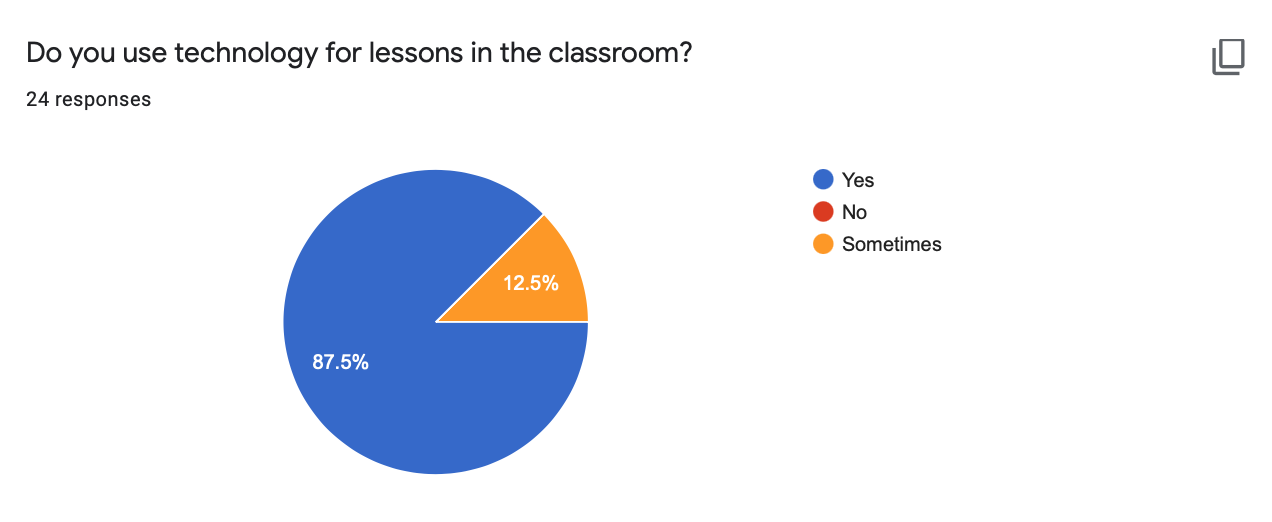
\includegraphics[width=1.0\textwidth]{IDD_LauraMartin_R00124705/Figures/8.png}
\caption{Pie chart representing the participants relationship with a person with Autism.}
{For question six, 24 respondents answered was technology used in the classroom, the highest response was yes at 87.5 percent and sometimes at 12.5 percent.}

\end{figure}

\begin{figure}[ht]
\centering
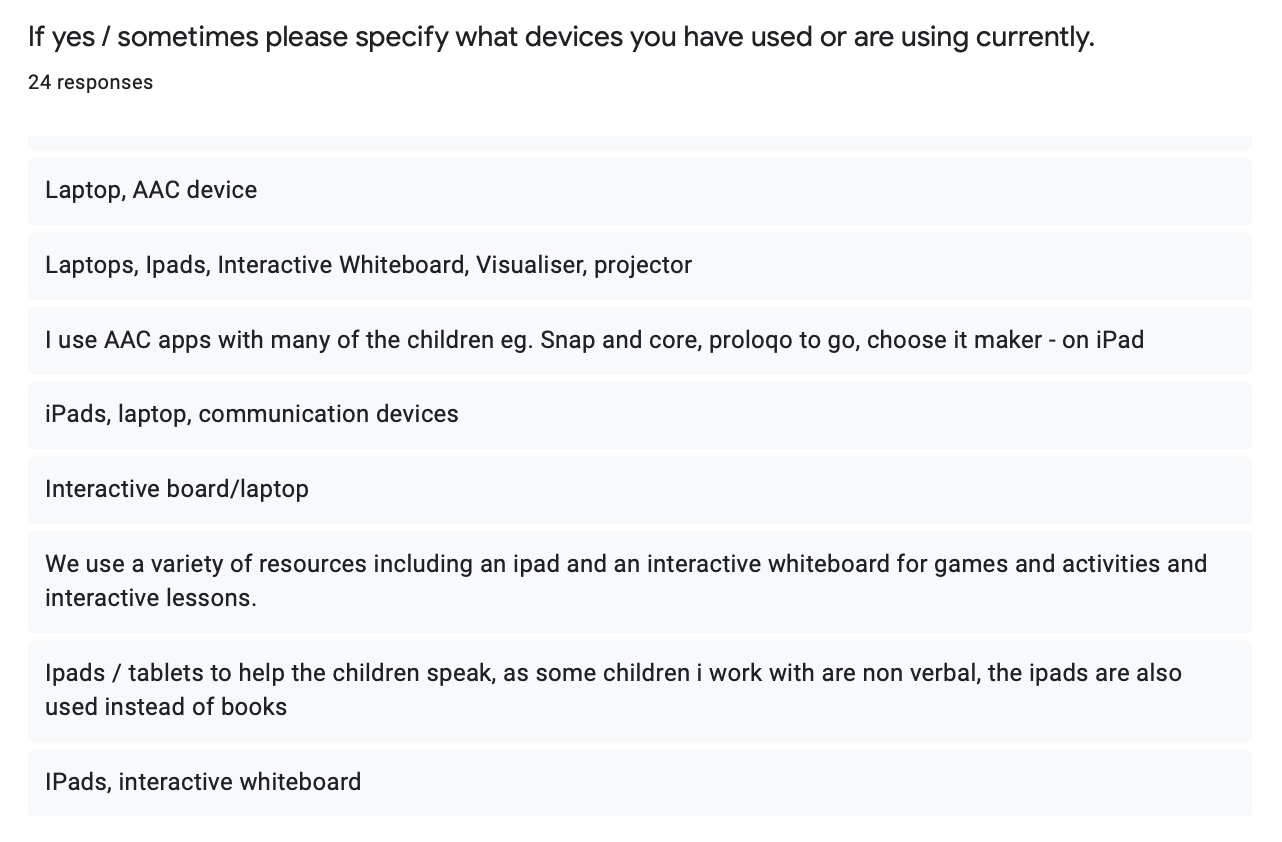
\includegraphics[width=1.0\textwidth]{IDD_LauraMartin_R00124705/Figures/9.png}
\caption{Technology and individuals in the classroom answer box}
{For question seven, 24 participants specified what technology they used in the classroom.}

\end{figure}

\begin{figure}[ht]
\centering
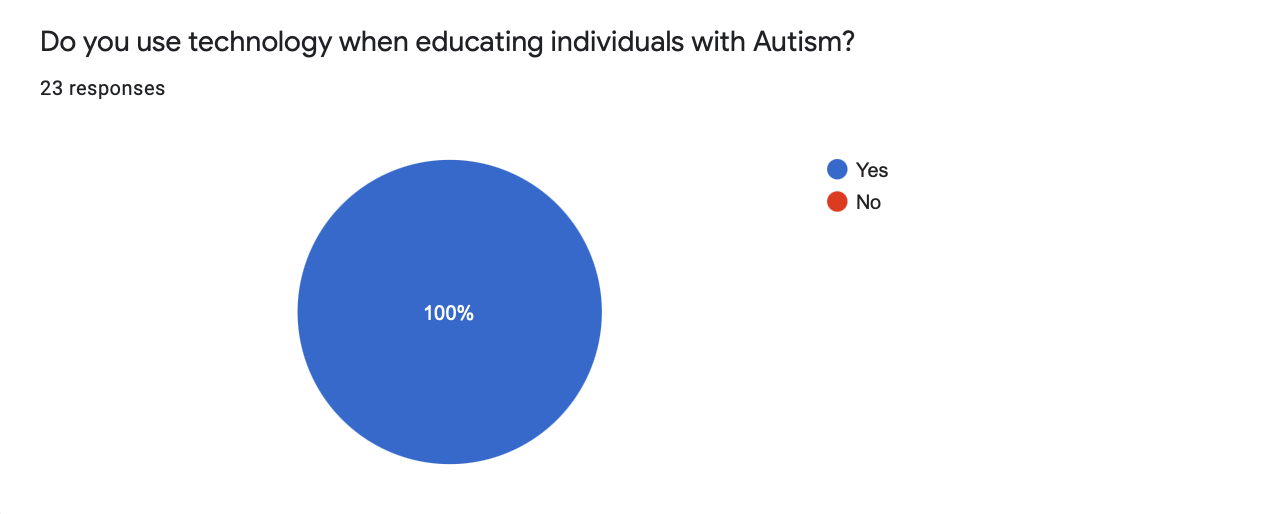
\includegraphics[width=1.0\textwidth]{IDD_LauraMartin_R00124705/Figures/10.png}
\caption{Technology and individuals with Autism pie chart}
{For question eight, 23 respondents answered a multiple choice question asking was technology used when educating individuals with Autism, yes was the response for all participants.}
\end{figure}

\begin{figure}[ht]
\centering
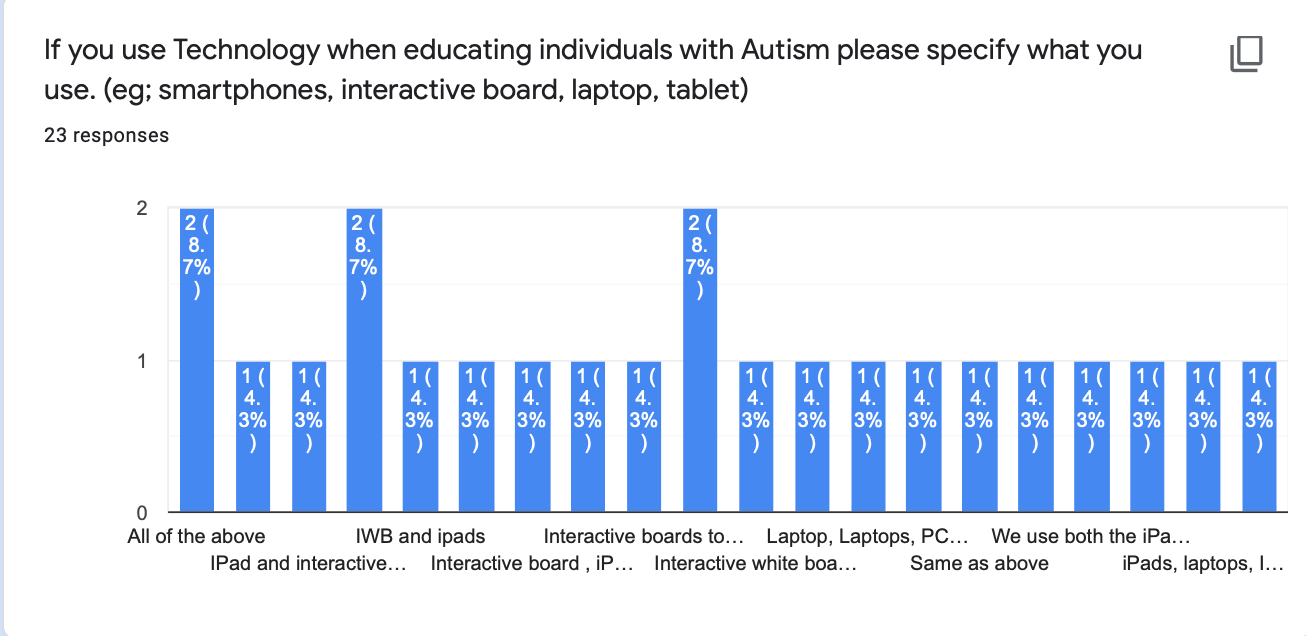
\includegraphics[width=1.0\textwidth]{IDD_LauraMartin_R00124705/Figures/11.png}
\caption{Technology used answer box}
{For question nine, 23 respondents answered what what technology they used when educating a student with Autism.}
\end{figure}

\begin{figure}[ht]
\centering
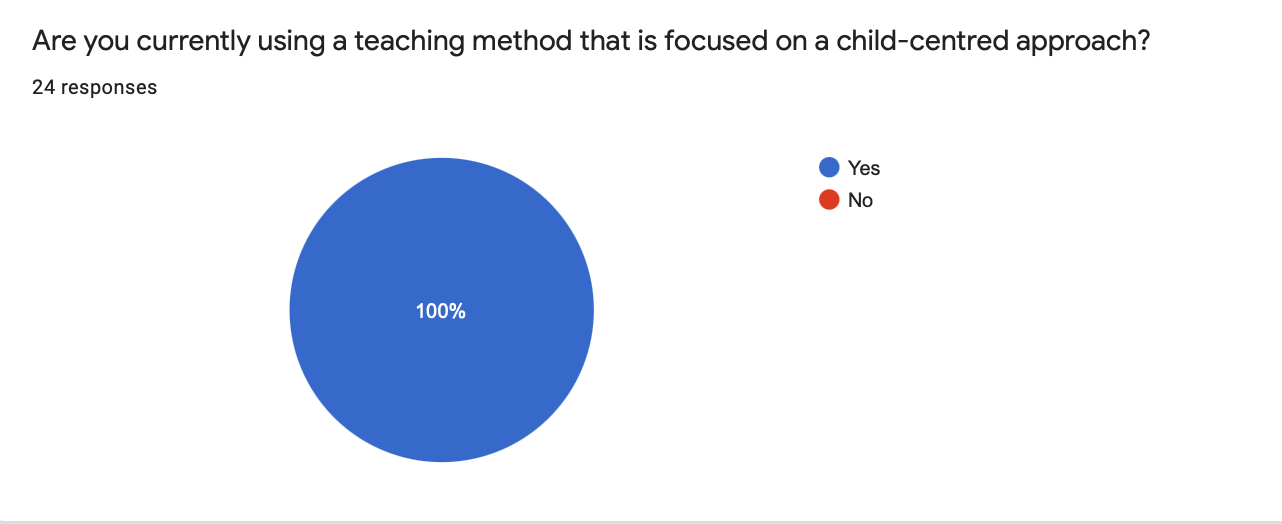
\includegraphics[width=1.0\textwidth]{IDD_LauraMartin_R00124705/Figures/12.png}
\caption{Child centered approach pie chart}
{For question ten, 24 respondents were asked if they used a child centered approach in the classroom, all participants answered yes.}
\end{figure}

\begin{figure}[ht]
\centering
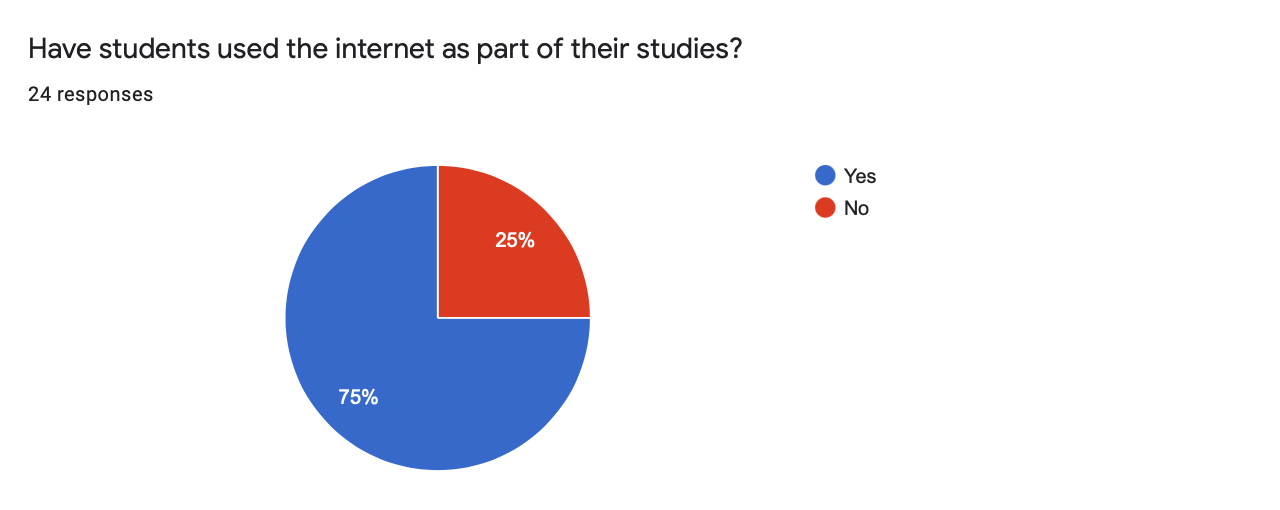
\includegraphics[width=1.0\textwidth]{IDD_LauraMartin_R00124705/Figures/13.png}
\caption{Students using the internet as part of studies pie chart}
{For question eleven, 24 respondents were given a multiple choice question asking if they used the internet as part of their studies, 75 percent answered yes and 25 percent answered no.}
\end{figure}

\begin{figure}[ht]
\centering
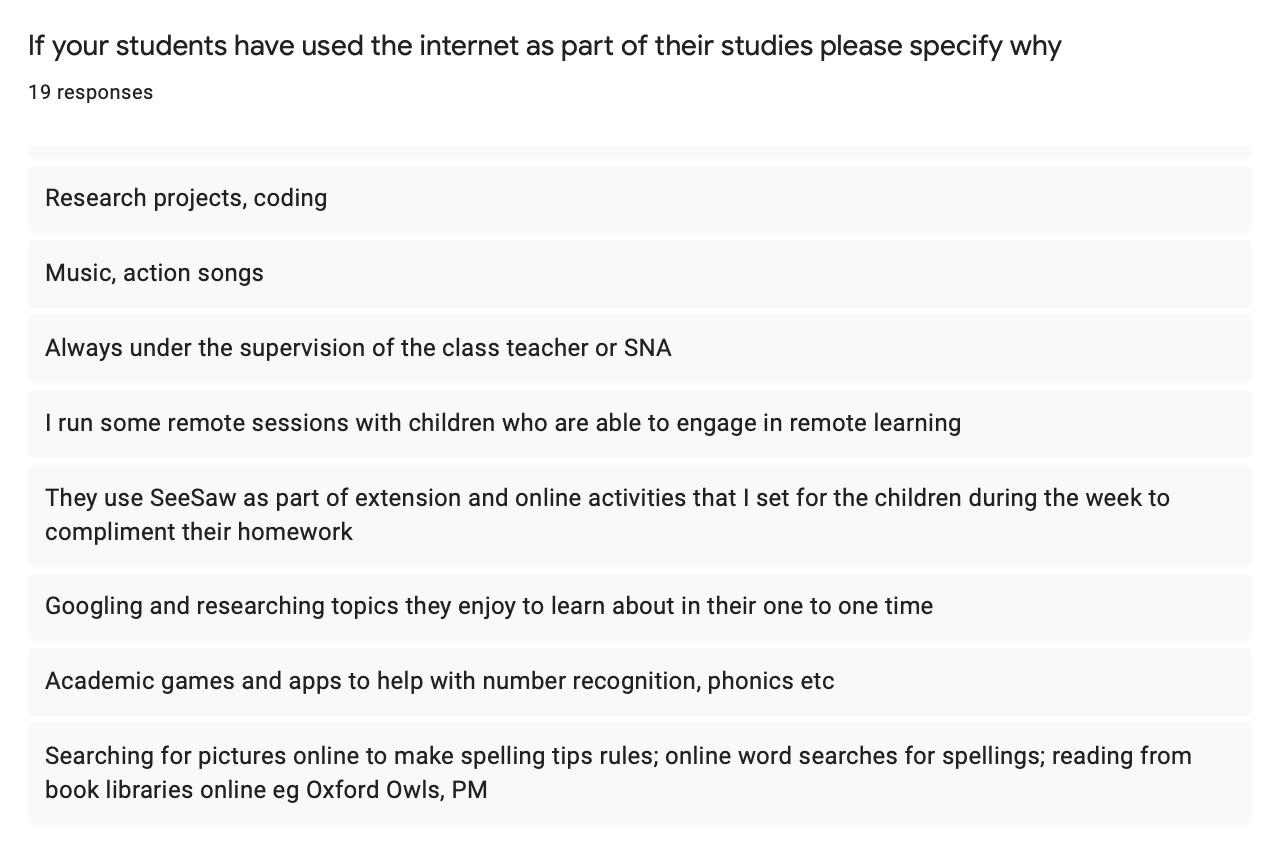
\includegraphics[width=1.0\textwidth]{IDD_LauraMartin_R00124705/Figures/14.png}
\caption{Internet used for studies answer box}
{For question Twelve, 19 respondents details on why their students use the internet as part of their studies.}
\end{figure}

\begin{figure}[ht]
\centering
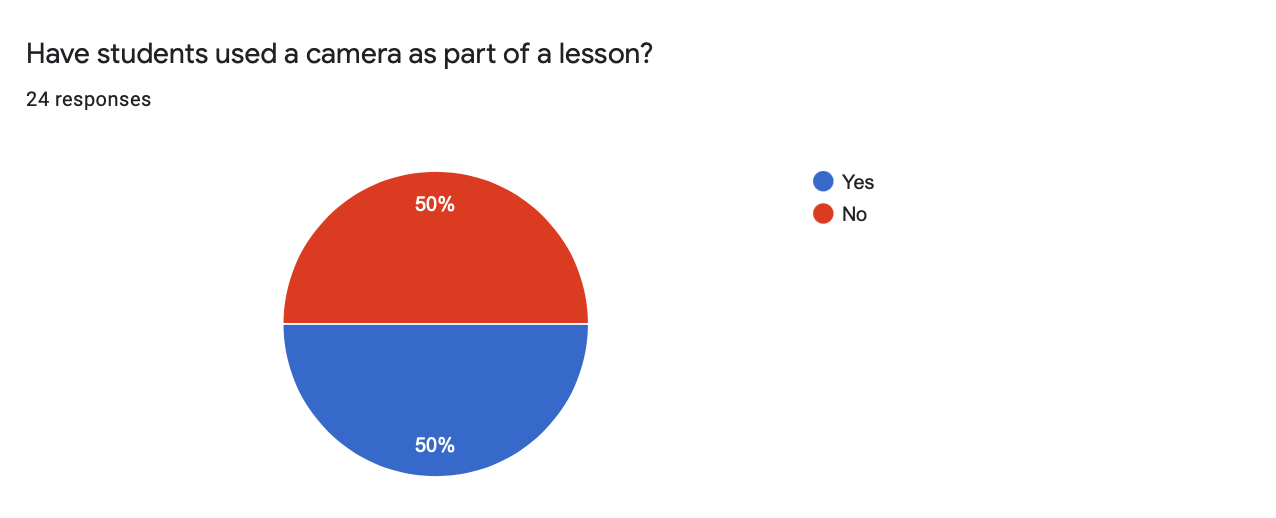
\includegraphics[width=1.0\textwidth]{IDD_LauraMartin_R00124705/Figures/15.png}
\caption{Smartphone camera used during lessons pie chart}
{For question thirteen, 24 respondents answered is their students used a camera as part of a lesson, 50 percent said yes and 50 percent said no.}
\end{figure}

\begin{figure}[ht]
\centering
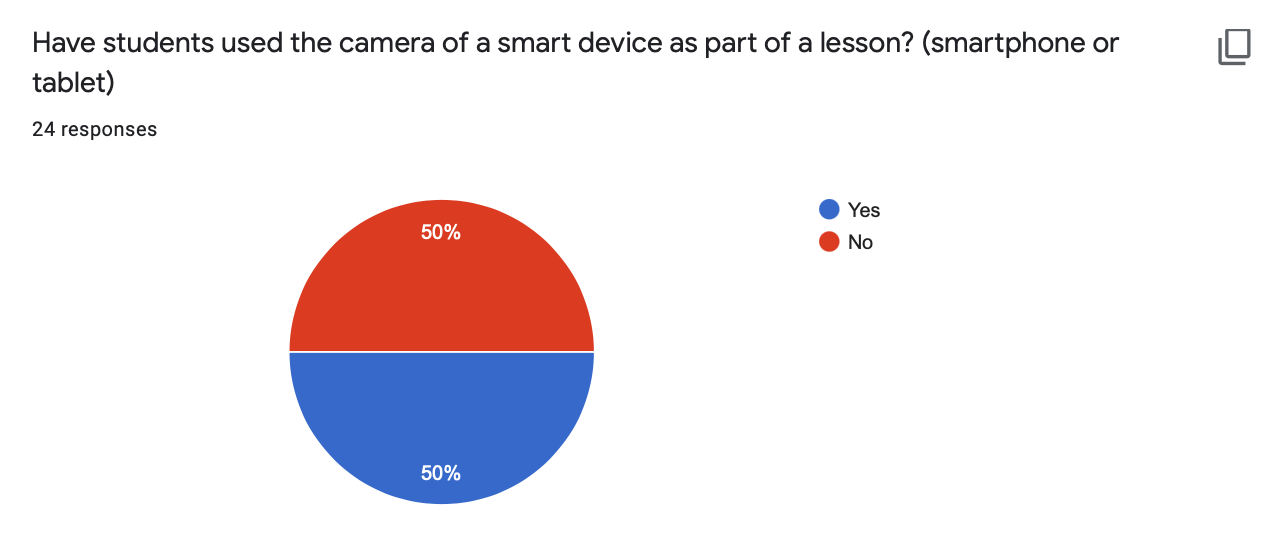
\includegraphics[width=1.0\textwidth]{IDD_LauraMartin_R00124705/Figures/16.png}
\caption{Use of a camera on a smart device during lessons pie chart}
{For question thirteen, 24 respondents answered is their students used a smartphone camera as part of a lesson, 50 percent said yes and 50 percent said no.}
\end{figure}

\begin{figure}[ht]
\centering
\includegraphics[width=1.0\textwidth]{IDD_LauraMartin_R00124705/Figures/17.1.png}
\caption{Why have students used a camera on a smart device during lessons answer box}
{For question fourteen, 13 respondents answered why a student used a smartphone camera as part of a lesson.}
\end{figure}

\begin{figure}[ht]
\centering
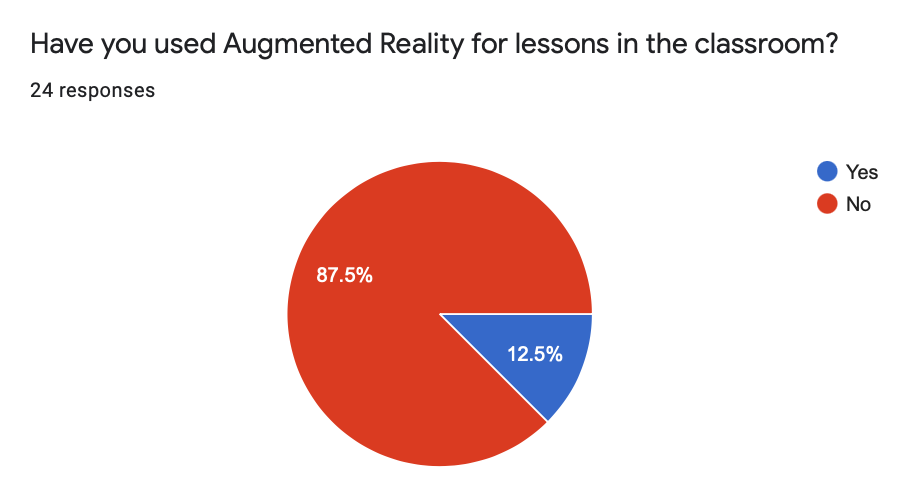
\includegraphics[width=1.0\textwidth]{IDD_LauraMartin_R00124705/Figures/17.png}
\caption{Use of AR in the classroom pie chart}
{For question fifteen, 24 respondents answered if they used AR for lessons in the classroom, 87.5 percent said no and 12.5 percent said yes.}
\end{figure}

\begin{figure}[ht]
\centering
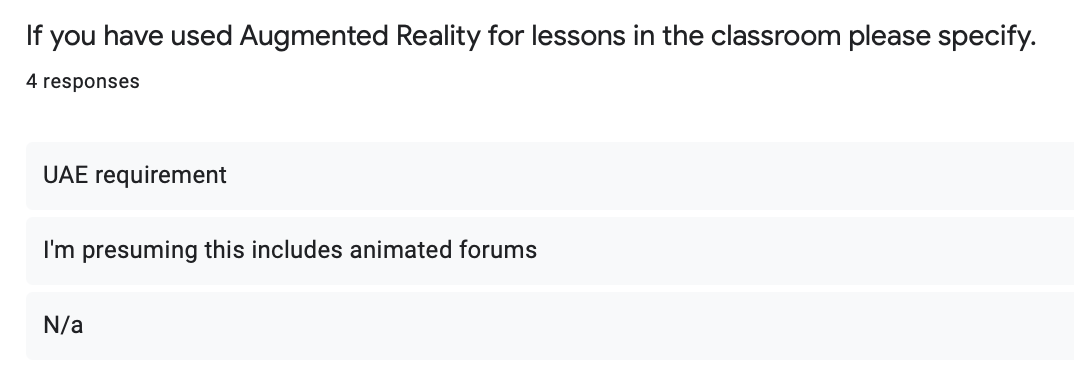
\includegraphics[width=1.0\textwidth]{IDD_LauraMartin_R00124705/Figures/18.png}
\caption{Use of AR in the classroom answer box}
{For question sixteen, 4 respondents explained why they have used AR in the classroom.}

\end{figure}

\begin{figure}[ht]
\centering
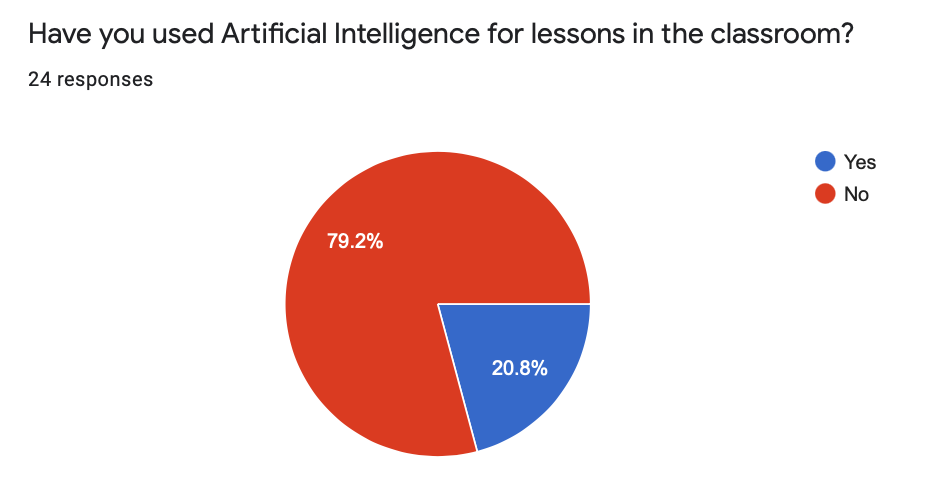
\includegraphics[width=1.0\textwidth]{IDD_LauraMartin_R00124705/Figures/19.png}
\caption{Use of AI pie chart}
{For question seventeen, 24 respondents answered if they used AI for lessons in the classroom, 79.2 percent said no and 20.8 percent said yes.}
\end{figure}

\begin{figure}[ht]
\centering
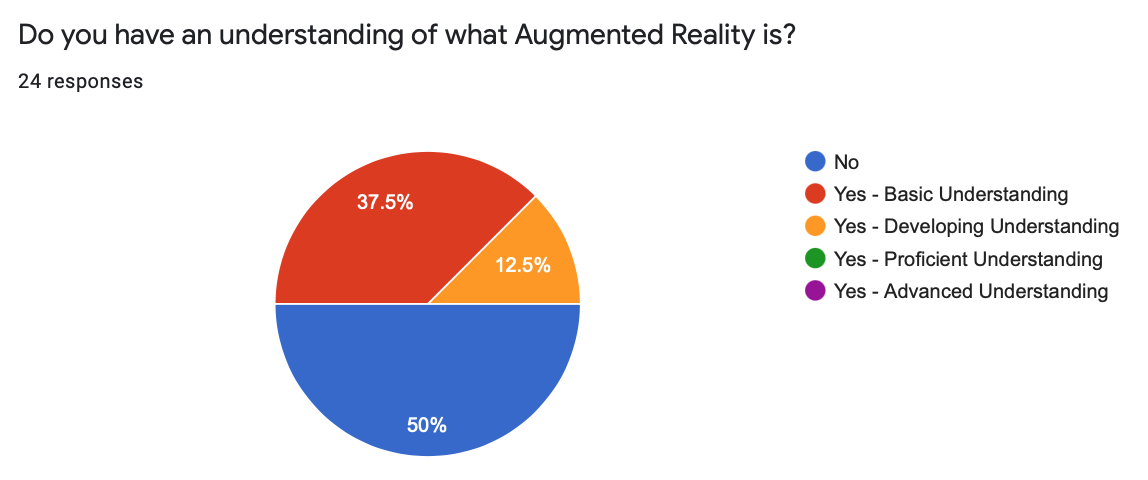
\includegraphics[width=1.0\textwidth]{IDD_LauraMartin_R00124705/Figures/20.png}
\caption{Participants understanding of AR pie chart}
{For question eighteen, 24 respondents were asked a multiple choice question asking if they had an understanding of AR, 50 percent of participants said no, 37.5 percent said yes and 12.5 percent said they had a developing understanding.}
\end{figure}

\begin{figure}[ht]
\centering
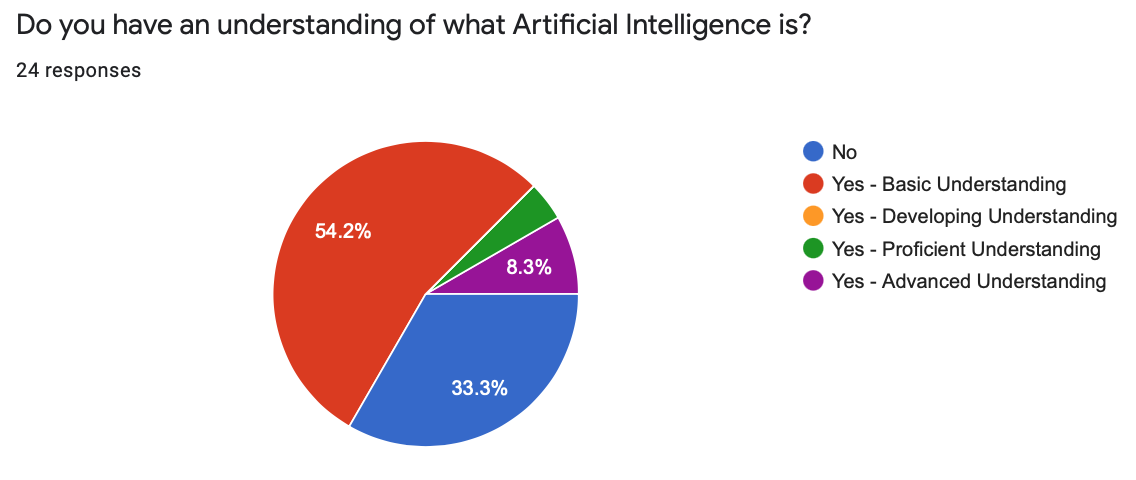
\includegraphics[width=1.0\textwidth]{IDD_LauraMartin_R00124705/Figures/21.png}
\caption{Participants understanding of AI pie chart}
{For question nineteen, 24 respondents were asked a multiple choice question asking if they had an understanding of AI, 33.3 percent of participants said no, 54.2 percent said yes - basic understanding, XX said yes - proficient understanding and 8.3 percent claim to have an advanced understanding of AI.}
\end{figure}

\begin{figure}[ht]
\centering
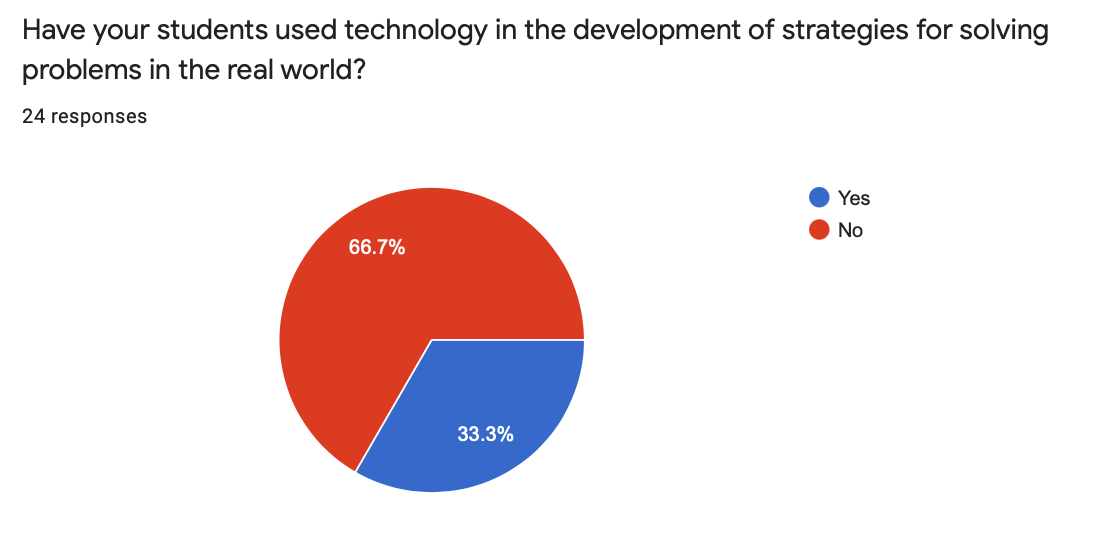
\includegraphics[width=1.0\textwidth]{IDD_LauraMartin_R00124705/Figures/22.png}
\caption{Students use of technology to solve real world problems pie chart}
{For question twenty, 24 respondents were asked if their students used technology to solve real world problems, 66.7 percent saud no and 33.3 percent said yes.}
\end{figure}

\begin{figure}[ht]
\centering
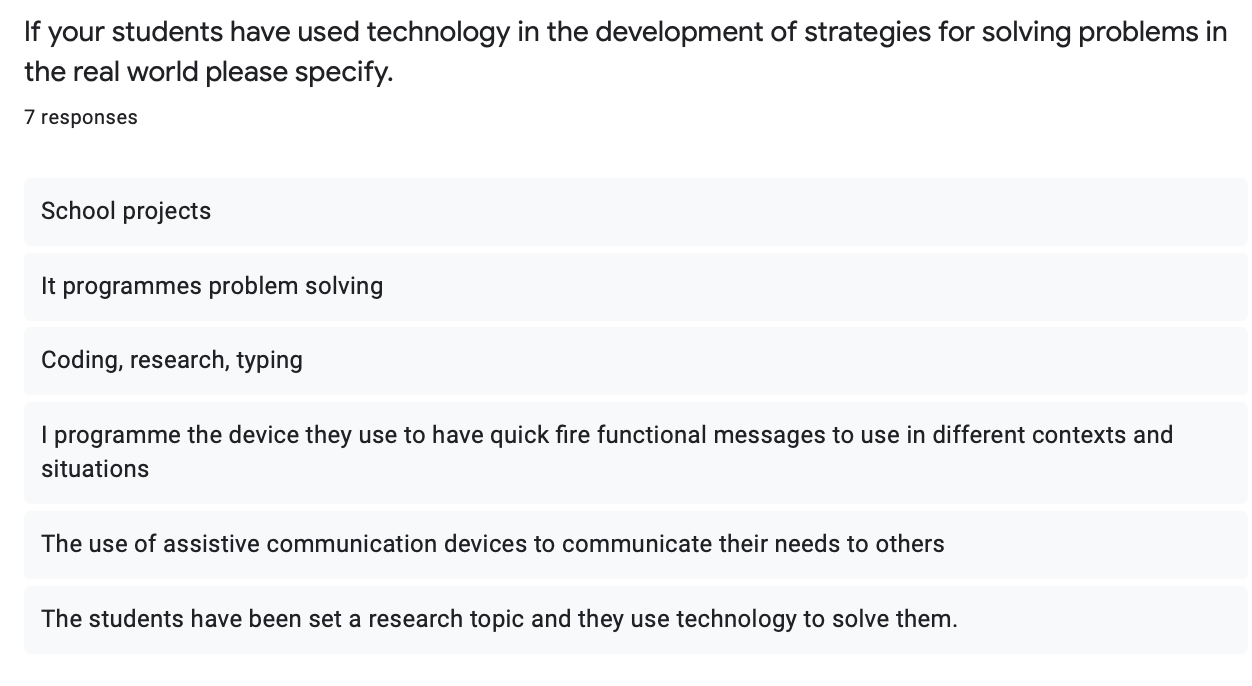
\includegraphics[width=1.0\textwidth]{IDD_LauraMartin_R00124705/Figures/23.png}
\caption{Students use of technology to solve real world problems answer box}
{For question twenty one, 7 respondents explained how their students used technology for real world problems.}
\end{figure}

\begin{figure}[ht]
\centering
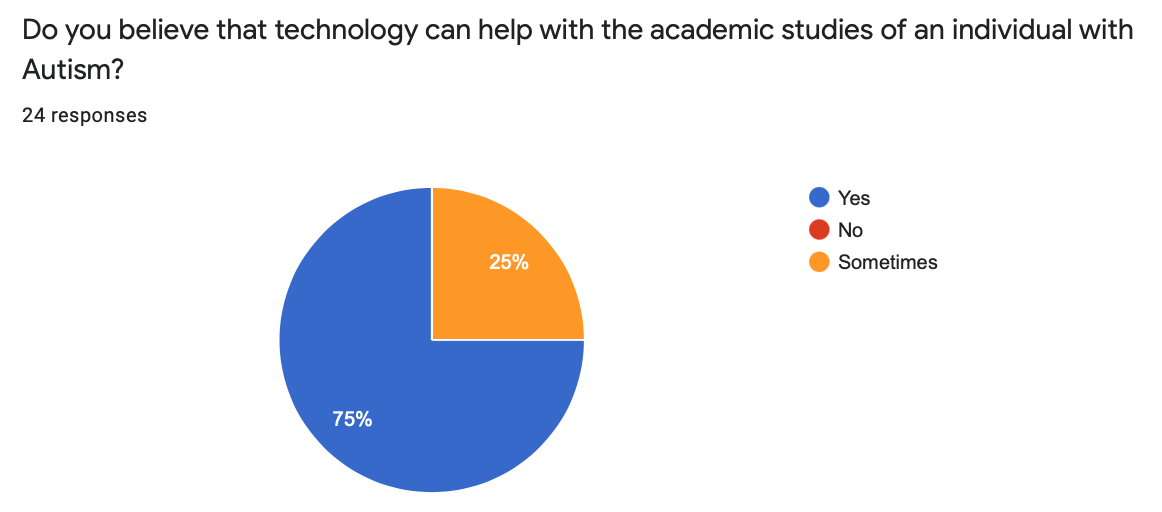
\includegraphics[width=1.0\textwidth]{IDD_LauraMartin_R00124705/Figures/24.png}
\caption{Technology and an Autistic individuals academic studies pie chart}
{For question twenty two, 24 were asked if they believe technology can help with the education of a student with Autism. 75 percent of the participants said yes and 25 percent said sometimes.}
\end{figure}

\begin{figure}[ht]
\centering
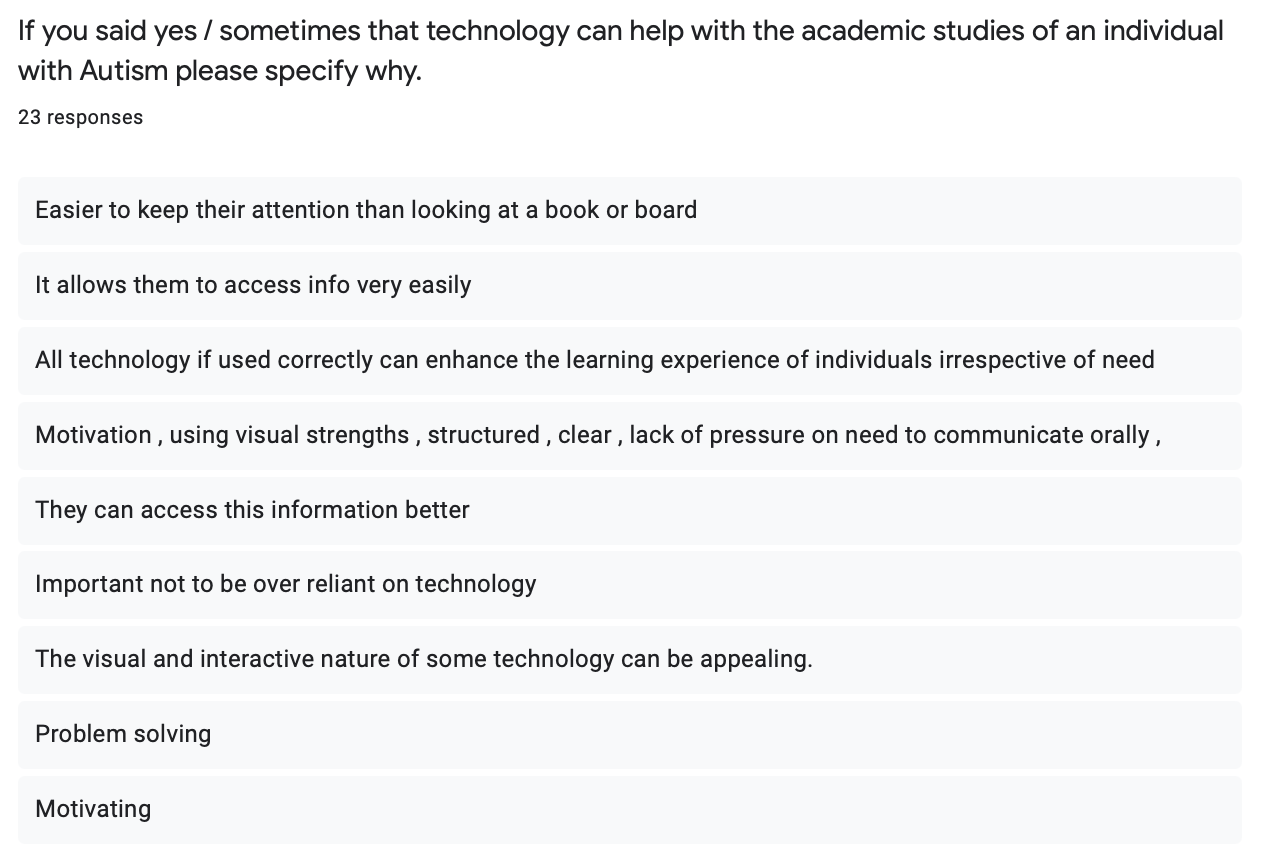
\includegraphics[width=1.0\textwidth]{IDD_LauraMartin_R00124705/Figures/25.png}
\caption{Technology and an Autistic individuals academic studies answer box}
{For question twenty three, 23 respondents gave feedback on how technology can help with the academic studies of an individual with Autism.}
\end{figure}

\begin{figure}[ht]
\centering
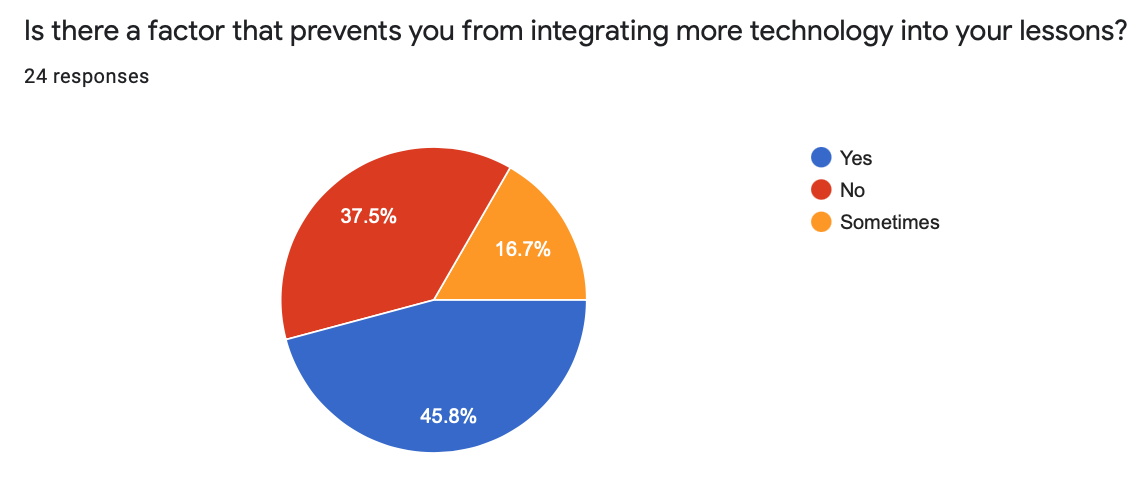
\includegraphics[width=1.0\textwidth]{IDD_LauraMartin_R00124705/Figures/26.png}
\caption{More technology integration pie chart}
{For question twenty four, 24 respondents were asked a multiple choice question of factors that could prevent them from integrating more technology into their lessons. 45.8 percent said yes, 37.5 percent said no and 16.7 percent said sometimes.}
\end{figure}

\begin{figure}[ht]
\centering
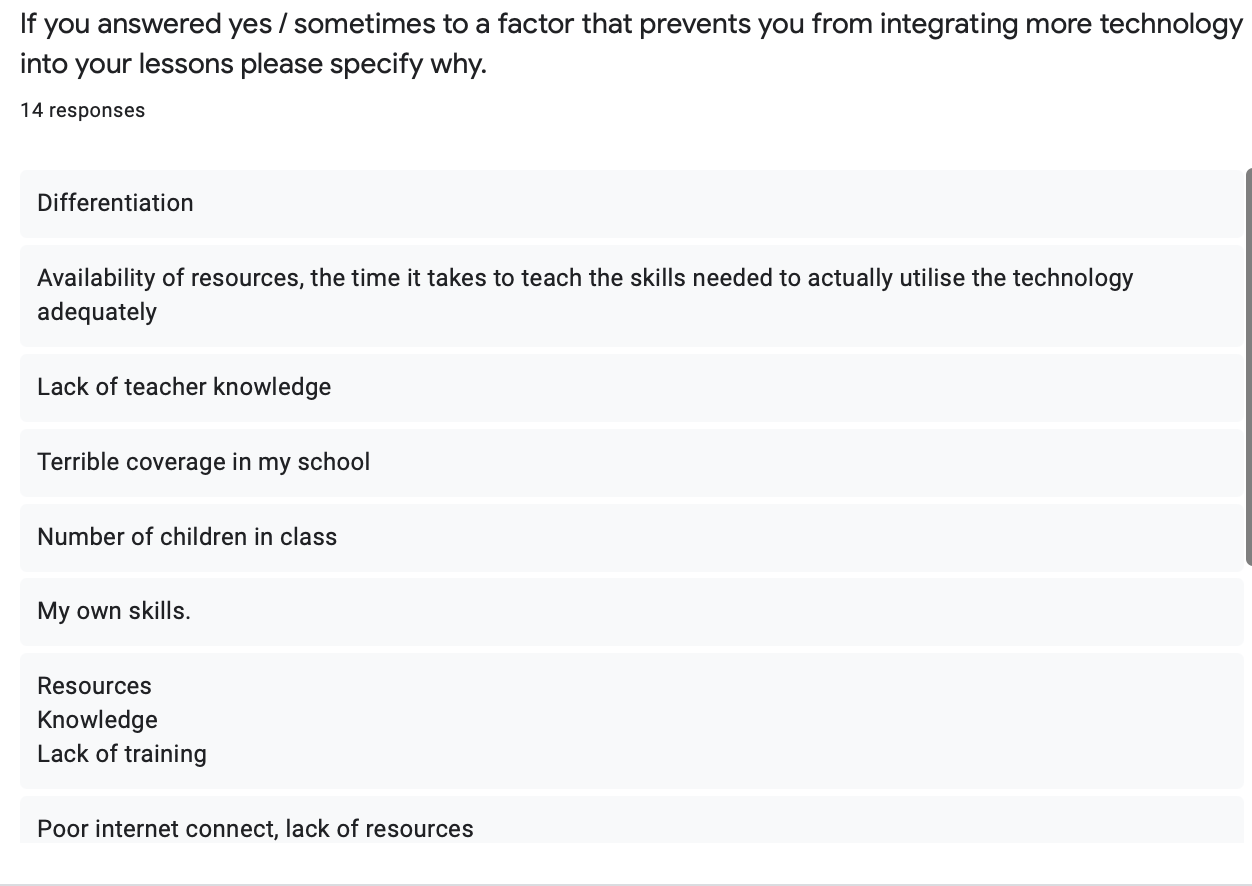
\includegraphics[width=1.0\textwidth]{IDD_LauraMartin_R00124705/Figures/27.png}
\caption{More technology integration answer box}
{For question twenty five, 14 respondents gave information as to why they have or sometimes have factors that prevent them using more technology in their lessons.}
\end{figure}

\begin{figure}[ht]
\centering
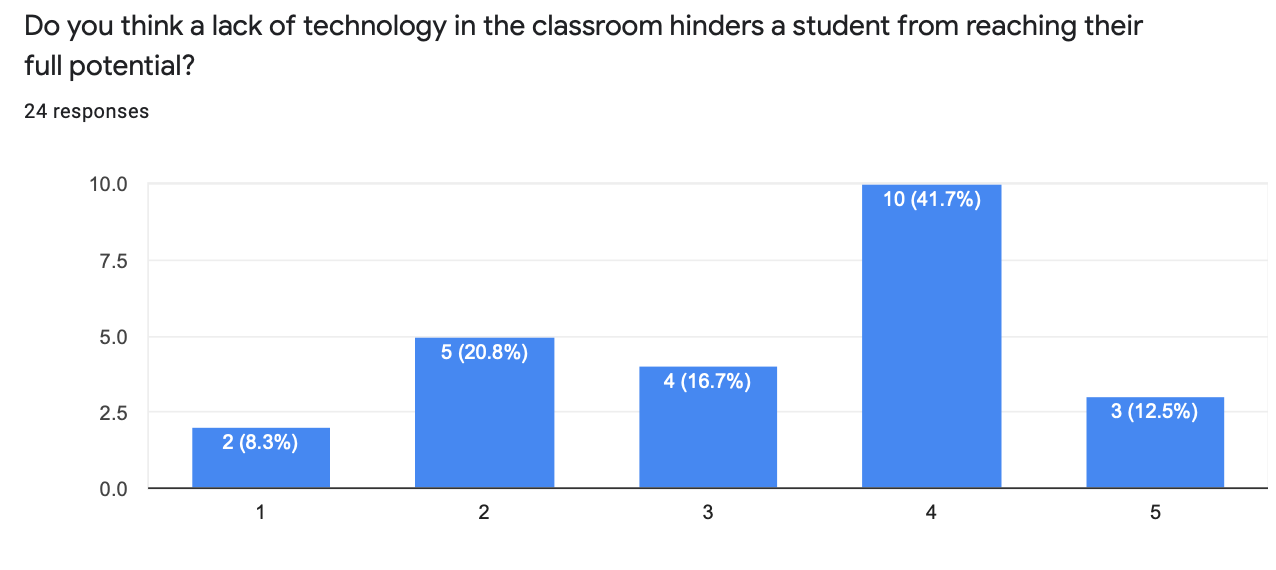
\includegraphics[width=1.0\textwidth]{IDD_LauraMartin_R00124705/Figures/28.png}
\caption{Technology hindering a student from reaching their full potential liner graph}
{For question twenty six, 24 participants answered a linear graph asking do they think a lack of technology can hinder a student reaching their full potential, rank 1 is strongly disagree and rank 5 was strongly agree.}
\end{figure}

\begin{figure}[ht]
\centering
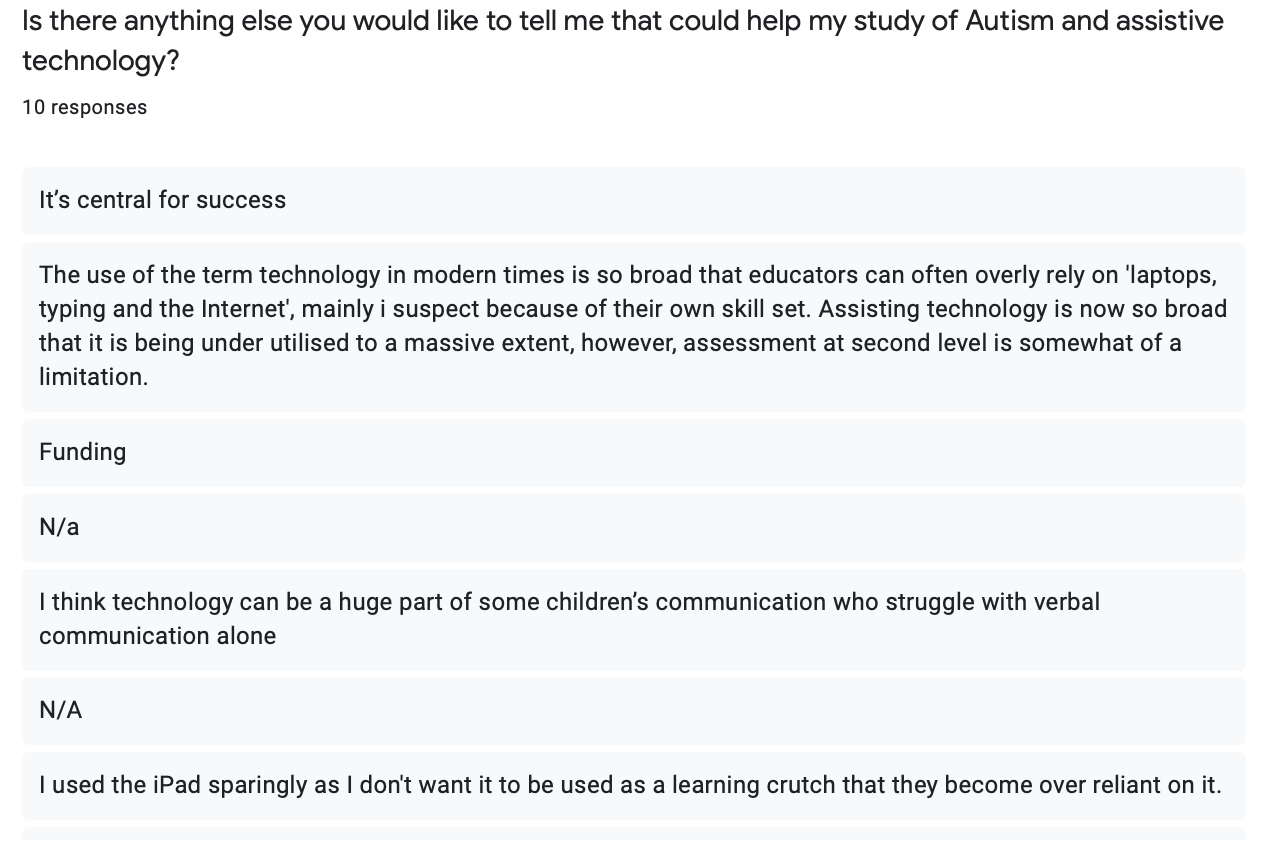
\includegraphics[width=1.0\textwidth]{IDD_LauraMartin_R00124705/Figures/29.png}
\caption{Additional information for this study answer box}
{For question twenty seven, 11 respondents gave feedback that could improve the study going forwards.}
\end{figure}


%\newpage

\subsection{Survey one analysis}

\begin{table} [b]
    \centering
\begin{tabular}{ | m{3em} | m{10cm}| } 
\hline
Q1. & There is a good range of occupations that are related to the target audience. \\ 
\hline
Q.2 & This question gave the details of the participants, it concluded of their name and email address for further contact. \\ 
\hline
Q.3 & 100 percent of the participants educates a person with Autism, this is crucial for feedback and design going foreword.  \\ 
\hline
Q.4 & 83.3 percent of the respondents educated children with Autism who were the school going age of 4-11, this is vital information as that is the age of the demographic for the proposed application.  \\ 
\hline
Q.5 & 83.3 percent of the respondents educated children in a mixed gender school, while 16.7 percent taught in a all male school. This is interesting feedback as none of the applicants educated in an all female school.  \\ 
\hline
Q.6 & 83.3 percent of the respondents claimed their students struggled with either their homework or their school work and 16.7 percent had some difficulty. This result was to be expected as the Children are learning new skills and having a learning disability typically can make this challenging.   \\ 
\hline
Q.7 & 87.5 percent of the participants use technology in the class while 12.5 percent only sometimes use technology, this can be put down to limitations, resources and internet connection in the school. \\ 
\hline
Q.8 & All respondents explained what devices they used in the classroom, the most common answer was a form of tablet and an interactive whiteboard. \\ 
\hline
Q.9 & 100 percent of the respondents used a form of technology for educating students with Autism. \\ 
\hline
Q.10 & The respondents explained what form of devices they used to educate a student with Autism, the most common answer was an interactive whiteboard and a form of table. \\ 
\hline
Q.11 & 100 percent of the respondents used a child centered approach when educating students with Autism, this is expected as it is a recommend form of practice for individuals with Autism as ability can vary. \\ 
\hline
Q.12 & 75 percent of respondents used the internet as part of their studies, while 25 percent did not. This is interesting as due to the COVID-19 pandemic all schools in Ireland for a period of time had to migrate to teaching online. \\ 
\hline

Q.13 & Respondents gave an explanation as to why students would access the internet as part of their studies, the main reasons were accessing information for a project, or using the internet to access the curriculum or SeeSaw, an online learning portal for schools.  \\
\hline
Q.14 & 50 percent of respondents used a camera as part of their studies, while 50 percent did not. This was interesting as half the respondents did not use a camera to track students progress while education was online.  \\
\hline
Q.15 & 50 percent of respondents used a smart device camera as part of their studies, while 50 percent did not. This is not surprising as the same results appeared in question 14.  \\
\hline
\end{tabular}
\centering

\caption{Survey one analysis}
    \label{tab:my_label}
\end{table}


\begin{table} [b]
    \centering
\begin{tabular}{ | m{3em} | m{10cm}| } 
\hline
Q1. & There is a good range of occupations that are related to the target audience. \\ 
\hline
Q.2 & This question gave the details of the participants, it concluded of their name and email address for further contact. \\ 
\hline
Q.3 & 100 percent of the participants educates a person with Autism, this is crucial for feedback and design going foreword.  \\ 
\hline
Q.4 & 83.3 percent of the respondents educated children with Autism who were the school going age of 4-11, this is vital information as that is the age of the demographic for the proposed application.  \\ 
\hline
Q.5 & 83.3 percent of the respondents educated children in a mixed gender school, while 16.7 percent taught in a all male school. This is interesting feedback as none of the applicants educated in an all female school.  \\ 
\hline
Q.6 & 83.3 percent of the respondents claimed their students struggled with either their homework or their school work and 16.7 percent had some difficulty. This result was to be expected as the Children are learning new skills and having a learning disability typically can make this challenging.   \\ 
\hline
Q.7 & 87.5 percent of the participants use technology in the class while 12.5 percent only sometimes use technology, this can be put down to limitations, resources and internet connection in the school. \\ 
\hline
Q.8 & All respondents explained what devices they used in the classroom, the most common answer was a form of tablet and an interactive whiteboard. \\ 
\hline
Q.9 & 100 percent of the respondents used a form of technology for educating students with Autism. \\ 
\hline
Q.10 & The respondents explained what form of devices they used to educate a student with Autism, the most common answer was an interactive whiteboard and a form of table. \\ 
\hline
Q.11 & 100 percent of the respondents used a child centered approach when educating students with Autism, this is expected as it is a recommend form of practice for individuals with Autism as ability can vary. \\ 
\hline
Q.12 & 75 percent of respondents used the internet as part of their studies, while 25 percent did not. This is interesting as due to the COVID-19 pandemic all schools in Ireland for a period of time had to migrate to teaching online. \\ 
\hline

Q.13 & Respondents gave an explanation as to why students would access the internet as part of their studies, the main reasons were accessing information for a project, or using the internet to access the curriculum or SeeSaw, an online learning portal for schools.  \\
\hline
Q.14 & 50 percent of respondents used a camera as part of their studies, while 50 percent did not. This was interesting as half the respondents did not use a camera to track students progress while education was online.  \\
\hline
Q.15 & 50 percent of respondents used a smart device camera as part of their studies, while 50 percent did not. This is not surprising as the same results appeared in question 14.  \\
\hline
\end{tabular}
\centering
\caption{Survey one analysis}
    \label{tab:my_label}
\end{table}
